%% GENERATED by tools/from_docs.py from stepss-docs. Do not edit by hand:
%% edit the page named below in stepss-docs and regenerate.
%% source: stepss-docs/src/content/docs/models/injectors/converters.md

\chapter{Converter models}\label{doc:model-inj-conv}

Injector models for converter-interfaced units other than the WECC ones: a generic inverter-based generator, a photovoltaic unit, and grid-forming and grid-following converters. The WECC wind turbine and storage models are on \hyperref[doc:model-inj-wecc]{WECC Wind and Storage}.

The \texttt{INJEC} record these models are entered with, and the rules on model names, are on the \hyperref[doc:model-inj]{Injector Models} page.

\section{\texorpdfstring{IBG (\texttt{inj\_IBG}): Inverter-Based Generator (Generic IBR)}{IBG (inj\_IBG): Inverter-Based Generator (Generic IBR)}}\label{model-inj-conv:ibg-inj_ibg-inverter-based-generator-generic-ibr}

\subsection{Description}\label{model-inj-conv:description}

A generic inverter-based generation model suitable for representing aggregated distributed generation or any grid-following IBR. The model includes a Phase-Locked Loop (PLL), inner current control with active (\(I_p\)) and reactive (\(I_q\)) current commands, LVRT/HVRT logic with voltage-dependent reactive current injection, frequency-responsive active power modulation, and reconnection logic after disconnection events.

\begin{figure}[htbp]
\centering
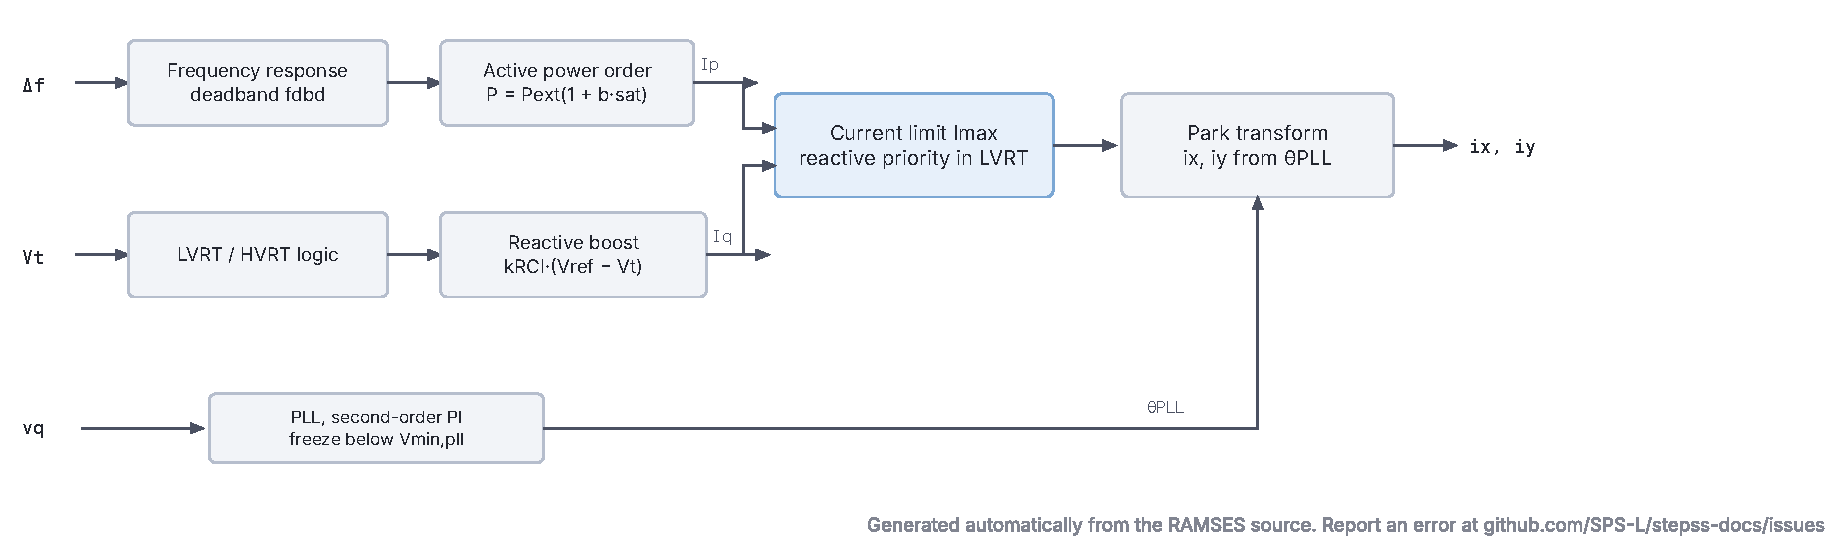
\includegraphics[width=0.98\linewidth]{figures/inj-ibg-light}
\caption{Generic inverter-based generator block diagram.}
\end{figure}

\subsection{Scientific Description}\label{model-inj-conv:scientific-description}

The PLL tracks the terminal voltage angle \(\theta\) via a second-order PI controller with a freeze option below \(V_{\mathrm{min,pll}}\):

\[\frac{d\theta_{\mathrm{PLL}}}{dt} = \Delta\omega_{\mathrm{PLL}}, \qquad \frac{d\Delta\omega_{\mathrm{PLL}}}{dt} = k_{\mathrm{PLL}}\, v_q\]

where \(v_q\) is the \(q\)-axis terminal voltage in the PLL frame. The current commands \(I_{p,\mathrm{cmd}}\) and \(I_{q,\mathrm{cmd}}\) are derived from outer controls:

\begin{itemize}
\item
  Active power is modulated by frequency according to frequency deadband \texttt{fdbd}:
  \[P = P_{\mathrm{ext}}\left(1 + b\,\mathrm{sat}(\Delta f - f_{\mathrm{start}}, f_{\mathrm{min}}, f_{\mathrm{max}})\right)\]
\item
  During voltage dips (LVRT), reactive current is boosted:
  \[I_{q,\mathrm{boost}} = k_{\mathrm{RCI}}\,(V_{\mathrm{ref}} - V_t)\]
\item
  Current magnitude is limited to \(I_{\mathrm{max}}\) with priority to reactive current during LVRT.
\end{itemize}

The injected currents in \(x\)-\(y\) frame are:

\[i_x = I_p \cos\theta_{\mathrm{PLL}} - I_q \sin\theta_{\mathrm{PLL}}\]
\[i_y = I_p \sin\theta_{\mathrm{PLL}} + I_q \cos\theta_{\mathrm{PLL}}\]

\subsection{Parameters}\label{model-inj-conv:parameters}

\begin{small}\begin{longtable}[]{@{}llll@{}}
\toprule\noalign{}
\# & Name & Description & Unit \\
\midrule\noalign{}
\endhead
\bottomrule\noalign{}
\endlastfoot
1 & \texttt{Imax} & Maximum current magnitude & pu \\
2 & \texttt{IN} & Nominal current & pu \\
3 & \texttt{Iprate} & Active current ramp rate & pu/s \\
4 & \texttt{Tg} & Generator time constant & s \\
5 & \texttt{Tm} & Measurement filter time constant & s \\
6 & \texttt{tLVRT1} & LVRT ride-through time threshold 1 & s \\
7 & \texttt{tLVRT2} & LVRT ride-through time threshold 2 & s \\
8 & \texttt{tLVRTint} & LVRT integration time & s \\
9 & \texttt{Vmax} & Maximum voltage for operation & pu \\
10 & \texttt{tau} & PLL response time & ms \\
11 & \texttt{Vminpll} & Voltage below which PLL is frozen & pu \\
12 & \texttt{a} & LVRT voltage-current curve slope & \\
13 & \texttt{Vmin} & Minimum LVRT voltage & pu \\
14 & \texttt{Vint} & Intermediate LVRT voltage & pu \\
15 & \texttt{fmin} & Minimum frequency for operation & pu \\
16 & \texttt{fmax} & Maximum frequency for operation & pu \\
17 & \texttt{fstart} & Frequency threshold for P modulation & pu \\
18 & \texttt{b} & Frequency droop gain & \\
19 & \texttt{fr} & Reference frequency & pu \\
20 & \texttt{Tr} & Reconnection delay after trip & s \\
21 & \texttt{Re} & Grid equivalent resistance & pu \\
22 & \texttt{Xe} & Grid equivalent reactance & pu \\
23 & \texttt{CM1} & LVRT control mode flag & \\
24 & \texttt{kRCI} & Reactive current injection gain (LVRT) & \\
25 & \texttt{kRCA} & Reactive current absorption gain (HVRT) & \\
26 & \texttt{m} & Active-reactive current priority parameter & \\
27 & \texttt{n} & Active-reactive current priority parameter & \\
28 & \texttt{dbmin} & Frequency deadband lower limit & pu \\
29 & \texttt{dbmax} & Frequency deadband upper limit & pu \\
30 & \texttt{HVRT} & HVRT flag & \\
31 & \texttt{LVRT} & LVRT flag & \\
32 & \texttt{CM2} & Control mode 2 flag & \\
33 & \texttt{Vtrip} & Trip voltage threshold & pu \\
\end{longtable}\end{small}

\subsection{State Variables}\label{model-inj-conv:state-variables}

\begin{small}\begin{longtable}[]{@{}ll@{}}
\toprule\noalign{}
Variable & Description \\
\midrule\noalign{}
\endhead
\bottomrule\noalign{}
\endlastfoot
\texttt{vxl}, \texttt{vyl} & Filtered terminal voltage components \\
\texttt{Vt} & Terminal voltage magnitude \\
\texttt{PLLPhaseAngle} & PLL phase angle \\
\texttt{Vm} & Voltage magnitude measurement \\
\texttt{Ip}, \texttt{Iq} & Active and reactive current outputs \\
\texttt{Ipcmd}, \texttt{Iqcmd} & Current commands \\
\texttt{Iqmax}, \texttt{Iqmin} & Reactive current limits \\
\texttt{Ipmax}, \texttt{Ipmin} & Active current limits \\
\texttt{DeltaW}, \texttt{DeltaWf} & Frequency deviation and filtered value \\
\texttt{Pgen}, \texttt{Qgen} & Generated active and reactive power \\
\end{longtable}\end{small}

\subsection{Usage Example}\label{model-inj-conv:usage-example}

\begin{Verbatim}
INJEC  IBG  IBG1  BUS_GEN
      # FP FQ P Q: share of the power-flow injection (FP, FQ) or initial power (P in MW, Q in Mvar)
      1.  0.  0.  0.
      # Imax: Maximum current magnitude (pu)
      1.1
      # IN: Nominal current (pu)
      1.0
      # Iprate: Maximum rate of rise of the active current, in multiples of IN (pu/s)
      0.5
      # Tg: Generator time constant (s)
      0.02
      # Tm: Measurement filter time constant (s)
      0.01
      # tLVRT1: LVRT trip delay for Vmin <= Vm < Vint (s)
      0.15
      # tLVRT2: LVRT trip delay at Vm = a, upper end of the linear ramp (s)
      1.5
      # tLVRTint: LVRT trip delay at Vm = Vint, lower end of the linear ramp (s)
      0.3
      # Vmax: Maximum voltage for operation (pu)
      1.2
      # tau: PLL response time (ms)
      20.0
      # Vminpll: Voltage below which PLL is frozen (pu)
      0.1
      # a: Voltage below which the LVRT timer runs; upper end of the LVRT curve (pu)
      0.9
      # Vmin: Minimum LVRT voltage (pu)
      0.1
      # Vint: Intermediate LVRT voltage (pu)
      0.3
      # fmin: Underfrequency trip threshold on the filtered frequency, 50 Hz system (Hz)
      47.5
      # fmax: Overfrequency trip threshold on the filtered frequency, 50 Hz system (Hz)
      51.5
      # fstart: Frequency above which active power is reduced (Hz)
      50.2
      # b: Overfrequency power reduction gain: fraction of initial P per pu frequency above fstart (pu/pu)
      20.0
      # fr: While the frequency stays at or above fr the power reduction is held at its maximum (Hz)
      50.05
      # Tr: Reconnection delay after trip (s)
      1.0
      # Re: Resistance between the terminal bus and the controlled converter-side voltage (pu)
      0.0
      # Xe: Reactance between the terminal bus and the controlled converter-side voltage (pu)
      0.05
      # CM1: 1 enables the m and kRCI injection below dbmin with reactive current limit IN; 0 disables
      1
      # kRCI: Reactive current injection gain below dbmin, in IN per pu voltage (pu/pu)
      2.0
      # kRCA: Reactive current absorption gain above dbmax, in IN per pu voltage (pu/pu)
      1.5
      # m: Step of reactive current injected below dbmin, in multiples of IN; needs CM1 or CM2 = 1 (pu)
      0.0
      # n: Step of reactive current absorbed above dbmax, in multiples of IN (pu)
      0.0
      # dbmin: Lower edge of the voltage dead-band; reactive injection and Q priority below it (pu)
      0.9
      # dbmax: Upper edge of the voltage dead-band; reactive absorption above it (pu)
      1.1
      # HVRT: 1 enables the kRCA absorption term above dbmax; 0 disables it
      1
      # LVRT: 1 uses Vmin and Vint as the LVRT curve breakpoints; 0 replaces both with Vtrip
      1
      # CM2: 1 enables the m and kRCI injection below dbmin with reactive current limit 0.707 Imax; 0 disables
      0
      # Vtrip: Undervoltage trip threshold, used only when LVRT = 0 (pu)
      0.85
;
\end{Verbatim}

\begin{center}\rule{0.5\linewidth}{0.5pt}\end{center}

\section{\texorpdfstring{PV (\texttt{inj\_PV}): Photovoltaic Generator}{PV (inj\_PV): Photovoltaic Generator}}\label{model-inj-conv:pv-inj_pv-photovoltaic-generator}

The data-file model name is \texttt{PV} (or \texttt{inj\_PV}).

\begin{docsnote}{Note}

Callable since 3.79. Earlier releases compiled this model under no name, so a data file referring to it was rejected.

\end{docsnote}

\subsection{Description}\label{model-inj-conv:description-1}

A photovoltaic generator model with similar WECC-derived structure to the wind turbine models. The model includes a plant controller (voltage/reactive power regulation), an electrical controller (current limits, LVRT), and generator/converter representation. Unlike wind turbines, there is no mechanical drive train; the active power set-point follows an irradiance input or a fixed reference. LVRT/HVRT logic and current limiting are identical to the Type 4 wind model.

\begin{figure}[htbp]
\centering
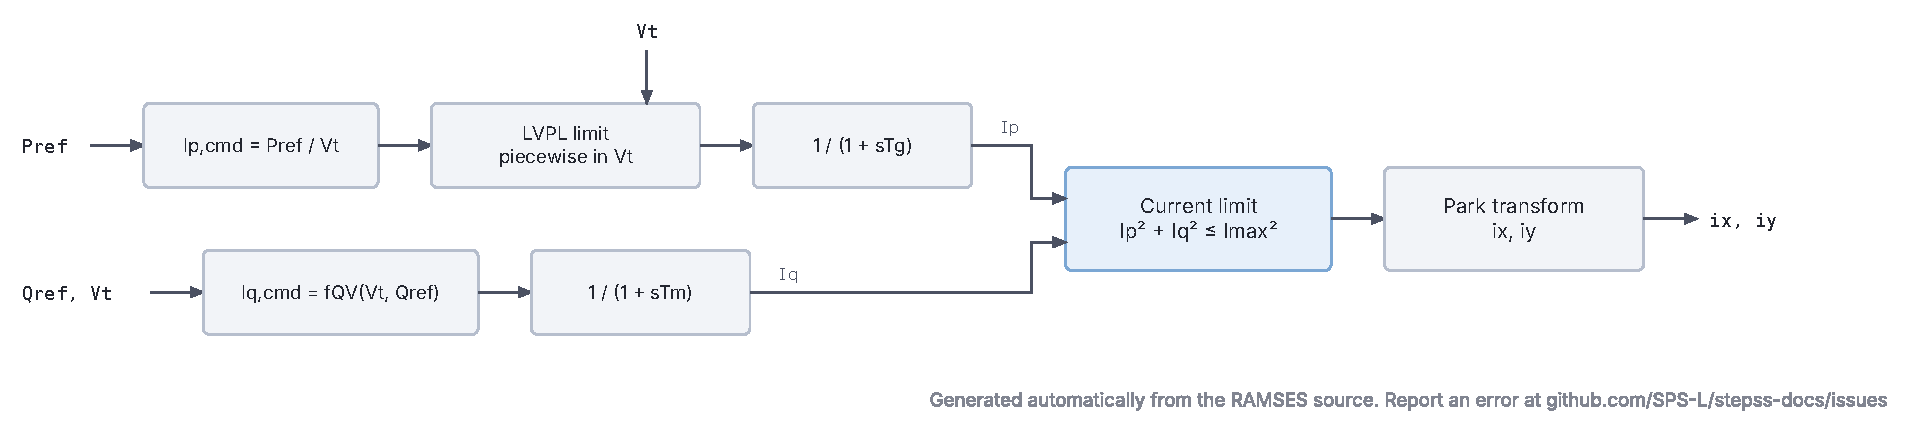
\includegraphics[width=0.98\linewidth]{figures/inj-pv-light}
\caption{Photovoltaic generator block diagram.}
\end{figure}

\subsection{Scientific Description}\label{model-inj-conv:scientific-description-1}

The PV generator delivers active and reactive power through current commands:

\[I_p = \frac{P_{\mathrm{ref}}}{V_t}, \qquad I_q = f_{\mathrm{QV}}(V_t, Q_{\mathrm{ref}})\]

subject to the constraint \(\sqrt{I_p^2 + I_q^2} \leq I_{\mathrm{max}}\). The inner current loop is a first-order filter:

\[T_g \frac{dI_p}{dt} = I_{p,\mathrm{cmd}} - I_p, \qquad T_m \frac{dI_q}{dt} = I_{q,\mathrm{cmd}} - I_q\]

Low-voltage power-logic (LVPL) limits active current during deep voltage sags via a piecewise-linear function of \(V_t\) with breakpoints \texttt{lvpnt0}, \texttt{lvpnt1}, \texttt{Lvpl1}. HVRT and LVRT timers control disconnection and reconnection.

\subsection{Parameters (selected)}\label{model-inj-conv:parameters-selected}

\begin{small}\begin{longtable}[]{@{}
  >{\raggedright\arraybackslash}p{(\linewidth - 8\tabcolsep) * \real{0.1599}}
  >{\raggedright\arraybackslash}p{(\linewidth - 8\tabcolsep) * \real{0.2391}}
  >{\raggedright\arraybackslash}p{(\linewidth - 8\tabcolsep) * \real{0.4695}}
  >{\raggedright\arraybackslash}p{(\linewidth - 8\tabcolsep) * \real{0.1315}}
@{}}
\toprule\noalign{}
\begin{minipage}[b]{\linewidth}\raggedright
\#
\end{minipage} & \begin{minipage}[b]{\linewidth}\raggedright
Name
\end{minipage} & \begin{minipage}[b]{\linewidth}\raggedright
Description
\end{minipage} & \begin{minipage}[b]{\linewidth}\raggedright
Unit
\end{minipage} \\
\midrule\noalign{}
\endhead
\bottomrule\noalign{}
\endlastfoot
1 & \texttt{Imax} & Maximum converter current & pu \\
2 & \texttt{IN} & Nominal current & pu \\
3 & \texttt{ratemax} & Reconnection ramp rate & pu/s \\
4 & \texttt{Tg} & Active current filter time constant & s \\
5 & \texttt{Tm} & Reactive current filter time constant & s \\
6--9 & LVRT timers & \texttt{tLVRT1}, \texttt{tLVRT2}, \texttt{tLVRTint}, \texttt{Vmax} & s, pu \\
10 & \texttt{kpll} & PLL gain & \\
11 & \texttt{Vminpll} & PLL freeze voltage & pu \\
12--14 & LVRT curve & \texttt{a}, \texttt{Vmin}, \texttt{Vint} & \\
21--22 & \texttt{Re}, \texttt{Xe} & Grid equivalent impedance & pu \\
23--29 & Current control & \texttt{CM1}, \texttt{kRCI}, \texttt{kRCA}, \texttt{m}, \texttt{n}, \texttt{dbmin}, \texttt{dbmax} & \\
34 & \texttt{BM} & Battery module flag & \\
\end{longtable}\end{small}

\subsection{Usage Example}\label{model-inj-conv:usage-example-1}

\begin{Verbatim}
INJEC  PV  PV1  BUS_PV
      # FP FQ P Q: share of the power-flow injection (FP, FQ) or initial power (P in MW, Q in Mvar)
      1.  1.  0.  0.
      # Imax: Maximum converter current; total current limit while Vm < 0.9 pu, and lower reactive current limit in normal operation (pu)
      1.1
      # IN: Nominal current; active and reactive current limit when Vm >= 0.9 pu, reactive absorption limit during a dip, and base of m and n (pu)
      1.0
      # ratemax: Maximum rate of rise of the active current Ip (decrease is not rate limited) (pu/s)
      0.5
      # Tg: Time constant of the active and reactive current lags (Ip and Iq) (s)
      0.02
      # Tm: Voltage measurement time constant (Vm and the voltage components used by the PLL) (s)
      0.01
      # tLVRT1: LVRT trip delay for Vmin <= Vm < Vint (s)
      0.15
      # tLVRT2: LVRT trip delay at Vm = a (upper end of the linear ramp) (s)
      1.5
      # tLVRTint: LVRT trip delay at Vm = Vint (lower end of the linear ramp up to tLVRT2 at Vm = a) (s)
      0.3
      # Vmax: Overvoltage threshold on the unfiltered voltage behind Re + jXe; reaching it trips the unit permanently (pu)
      1.2
      # kpll: PLL proportional gain from q-axis voltage to angle rate (integral gain fixed at zero) (rad/s/pu)
      20.0
      # Vminpll: Voltage below which the PLL angle is frozen (pu)
      0.1
      # a: Voltage below which the LVRT timer runs; upper end of the LVRT curve (pu)
      0.9
      # Vmin: LVRT curve: below this voltage the unit trips at once (used when LVRT = 1) (pu)
      0.1
      # Vint: LVRT curve intermediate voltage between the tLVRT1 plateau and the ramp (used when LVRT = 1) (pu)
      0.3
      # fmin: Underfrequency threshold on the filtered frequency; below it the unit trips permanently (Hz)
      47.5
      # fmax: Overfrequency threshold on the filtered frequency; above it the unit trips permanently (Hz)
      51.5
      # fstart: Frequency above which active power is reduced (Hz)
      50.2
      # b: Overfrequency active power reduction gain: fraction of initial P per pu frequency above fstart (50 Hz base) (pu/pu)
      20.0
      # fr: While filtered frequency >= fr the power reduction is held at its maximum; below fr it follows frequency again (Hz)
      50.05
      # Tr: Time the current output stays at zero after an LVRT trip before it is restored (at most 5 s takes effect) (s)
      1.0
      # Re: Resistance between the terminal bus and the controlled (converter side) voltage (pu)
      0.0
      # Xe: Reactance between the terminal bus and the controlled (converter side) voltage (pu)
      0.05
      # CM1: Reactive current injection mode 1: 1 enables the m and kRCI injection below dbmin, dip Iq limit Imax; 0 disables
      1
      # kRCI: Reactive current injection gain per pu voltage below dbmin (active if CM1, CM2 or CM3 is 1) (pu/pu)
      2.0
      # kRCA: Reactive current absorption gain per pu voltage above dbmax (active only if HVRT = 1) (pu/pu)
      1.5
      # m: Step reactive current injected below dbmin, as a multiple of IN (active if CM1, CM2 or CM3 is 1) (pu)
      0.0
      # n: Step reactive current absorbed above dbmax, as a multiple of IN (always active, independent of HVRT) (pu)
      0.0
      # dbmin: Lower edge of the voltage deadband on Vm; reactive injection below it (pu)
      0.9
      # dbmax: Upper edge of the voltage deadband on Vm; reactive absorption above it (pu)
      1.1
      # HVRT: 1 enables the kRCA absorption term above dbmax; 0 disables it (does not affect the Vmax trip)
      1
      # LVRT: 1 uses Vmin and Vint as LVRT curve breakpoints; 0 replaces both with 0.8 pu
      1
      # CM2: Reactive current injection mode 2: 1 enables m and kRCI injection and caps dip Iq at 0.707 Imax; 0 disables
      0
      # CM3: Reactive current injection mode 3: 1 enables m and kRCI injection, dip Iq limit sqrt(Imax^2 - Ipcmd^2) and a PI voltage term; 0 disables
      0
      # BM: Blocking mode: 1 zeroes the active current and drops the initial reactive current while Vm < 0.9 pu; 0 keeps both
      0
;
\end{Verbatim}

\begin{center}\rule{0.5\linewidth}{0.5pt}\end{center}

\section{\texorpdfstring{GFOR (\texttt{inj\_GFOR}): Grid-Forming Converter (VSM)}{GFOR (inj\_GFOR): Grid-Forming Converter (VSM)}}\label{model-inj-conv:gfor-inj_gfor-grid-forming-converter-vsm}

The data-file model name is \texttt{GFOR} (or \texttt{inj\_GFOR}).

\subsection{Description}\label{model-inj-conv:description-2}

A grid-forming voltage source converter implementing Virtual Synchronous Machine (VSM) dynamics, modelled under the phasor approximation. The converter is an MMC-type VSC connected to the grid through its transformer (no LC filter); the DC side is not modelled (the DC voltage is assumed constant) so the focus is on the AC grid dynamics.

The modulated voltage magnitude is held at its setpoint \(V_m^0\) in normal operation, while the phase angle \(\delta_m\) is driven by a synthetic swing equation with inertia emulation (\(H\)) and oscillation damping (\(D\)) against a PLL estimate of the grid frequency. Participation in primary frequency control is optional, through the droop \(R_{\mathrm{droop}}\). Overcurrents are limited by proportionally scaling the \(d\)-\(q\) current vector back to the \(I_{\mathrm{max}}\) circle with a small time constant.

\subsection{Scientific Description}\label{model-inj-conv:scientific-description-2}

\textbf{Reference frame.} The \(d\) axis is attached to the internal phase angle \(\delta_m\) of the modulated voltage. Voltages and currents at the point of common coupling are transformed as:

\[v_d = v_x\cos\delta_m + v_y\sin\delta_m, \qquad v_q = -v_x\sin\delta_m + v_y\cos\delta_m\]

with the analogous transformation for the converter-side currents \(i_{xt} = k\, i_x\), \(i_{yt} = k\, i_y\), where \(k = r\, S_{\mathrm{base}}/S_{\mathrm{nom}}\) converts to per-unit on the converter base.

\textbf{Transformer.} The voltage-current relationship across the connection transformer (resistance \(R\), inductance \(L\), ideal ratio \(r\)) in the \(d\)-\(q\) frame is:

\[v_{md} = \frac{v_d}{r} + R\, i_d - \omega_m L\, i_q, \qquad v_{mq} = \frac{v_q}{r} + R\, i_q + \omega_m L\, i_d\]

\textbf{PLL.} The PLL only serves to estimate the grid angular frequency \(\tilde{\omega}_g\) for the damping term. It is the same model as in the grid-following converter (see the \hyperref[model-inj-conv:gfol-inj_gfol-grid-following-converter]{PLL diagram there}), with PI gains derived from the time constant \(T_{\mathrm{pll}}\):

\[K_{p\omega} = \frac{10}{\omega_N T_{\mathrm{pll}}}, \qquad K_{i\omega} = \frac{25}{\omega_N T_{\mathrm{pll}}^2}, \qquad \omega_N = 2\pi f_N\]

The PLL is frozen (hysteresis) when the PCC voltage falls below 0.4 pu and reactivated when it recovers above 0.5 pu (fixed thresholds in this model).

\textbf{Active power and phase angle control (VSM).}

\begin{figure}[htbp]
\centering
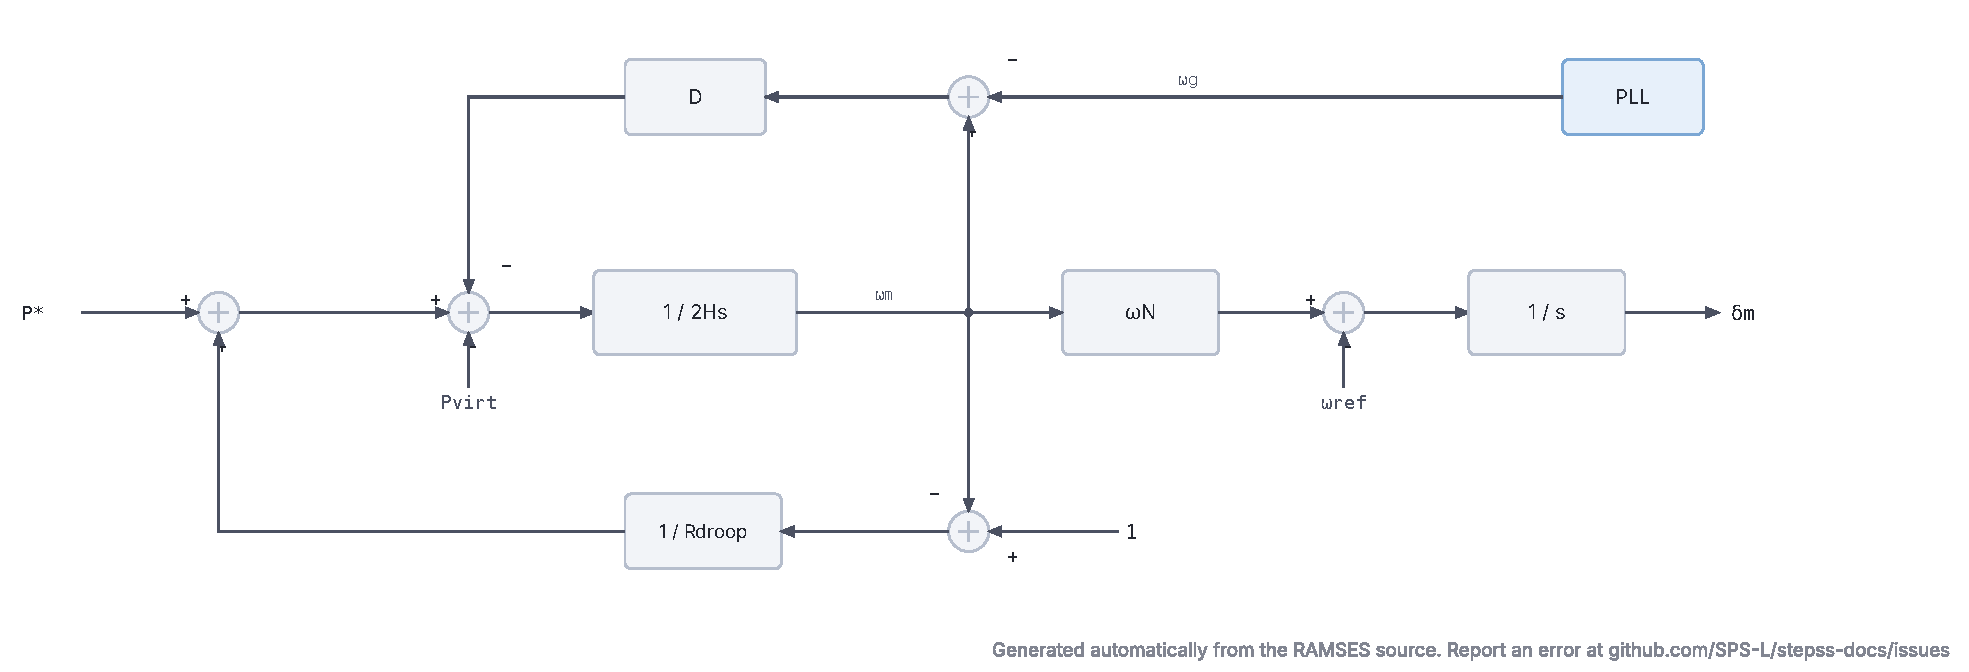
\includegraphics[width=0.98\linewidth]{figures/inj-gfor-vsm-light}
\caption{Grid-forming virtual synchronous machine block diagram.}
\end{figure}

\[2H\frac{d\omega_m}{dt} = P^* - P_{\mathrm{virt}} - D\left(\omega_m - \tilde{\omega}_g\right) + \frac{1 - \omega_m}{R_{\mathrm{droop}}}\]

\[\frac{d\delta_m}{dt} = \omega_N\left(\omega_m - \omega_{\mathrm{ref}}\right)\]

where \(P^*\) is the active power setpoint and \(P_{\mathrm{virt}}\) is the \emph{virtual power} computed from the \textbf{unsaturated} currents:

\[P_{\mathrm{virt}} = \frac{v_d}{r}\, i_d^* + \frac{v_q}{r}\, i_q^*\]

\(P_{\mathrm{virt}}\) equals the actual active power \(P\) when the current is not limited, and yields improved large-disturbance stability while the current is limited (the angle dynamics do not wind up).

\textbf{Current limitation.} The currents \((i_d^*, i_q^*)\) that would result from normal voltage control (i.e.~\(v_{md} = V_m^0\), \(v_{mq} = 0\)) are first determined from:

\[V_m^0 = \frac{v_d}{r} + R\, i_d^* - \omega_m L\, i_q^*, \qquad 0 = \frac{v_q}{r} + R\, i_q^* + \omega_m L\, i_d^*\]

The current overload ratio \(\rho = \sqrt{(i_d^*)^2 + (i_q^*)^2}\,/\,I_{\mathrm{max}}\) is passed through a first-order lag with time constant \(T_e\) (typically 1 ms) and a non-windup \textbf{lower limit of 1}, giving \(\rho_s\). Both current components are then decreased in the same proportion:

\[i_{ds}^* = \frac{i_d^*}{\rho_s}, \qquad i_{qs}^* = \frac{i_q^*}{\rho_s}\]

\begin{figure}[htbp]
\centering
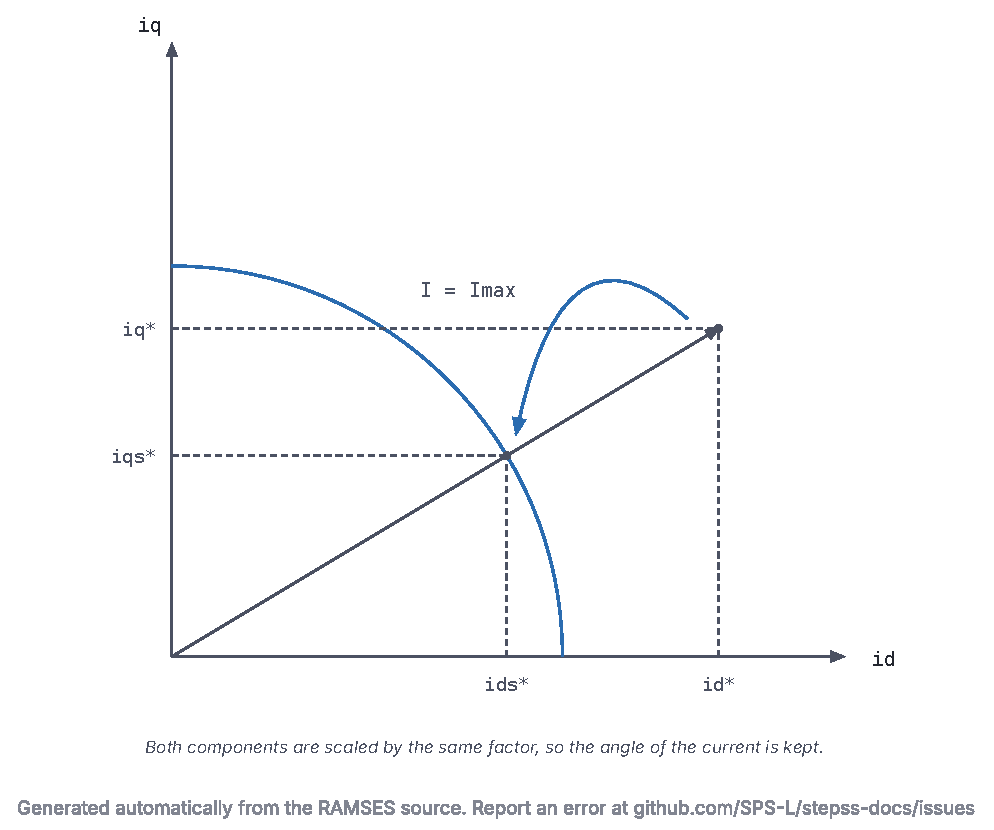
\includegraphics[width=0.98\linewidth]{figures/inj-gfor-currentlim-light}
\caption{Grid-forming current limitation.}
\end{figure}

and the modulated voltage is set to the value that yields the saturated currents:

\[v_{md} = \frac{v_d}{r} + R\, i_{ds}^* - \omega_m L\, i_{qs}^*, \qquad v_{mq} = \frac{v_q}{r} + R\, i_{qs}^* + \omega_m L\, i_{ds}^*\]

When \(I < I_{\mathrm{max}}\): \(\rho_s = 1\), the currents are unsaturated, and \(v_{md} = V_m^0\), \(v_{mq} = 0\).

\subsection{Parameters}\label{model-inj-conv:parameters-1}

Default values correspond to a 1100 MVA converter. Per-unit values refer to the nominal apparent power of the converter.

\begin{small}\begin{longtable}[]{@{}lllll@{}}
\toprule\noalign{}
\# & Name & Description & Unit & Default \\
\midrule\noalign{}
\endhead
\bottomrule\noalign{}
\endlastfoot
1 & \texttt{R} & Resistance of connection transformer & pu & 0.005 \\
2 & \texttt{L} & Inductance of connection transformer & pu & 0.15 \\
3 & \texttt{r} & Ratio of ideal transformer & & 1.02 \\
4 & \texttt{Snom} & Nominal apparent power & MVA & 1100 \\
5 & \texttt{H} & Inertia constant & s & 5.0 \\
6 & \texttt{D} & Damping constant of virtual synchronous machine & & 300 \\
7 & \texttt{Tpll} & Time constant of PLL & s & 0.1 \\
8 & \texttt{Rdroop} & Droop of primary frequency control & pu & 999 \\
9 & \texttt{Imax} & Maximum current (typically 1--1.2) & pu & 1.0 \\
10 & \texttt{Te} & Time constant of current saturation & s & 0.001 \\
\end{longtable}\end{small}

A very large \texttt{Rdroop} (e.g.~999) effectively disables participation in primary frequency control.

Five additional parameters are computed at initialization from the power-flow solution: \texttt{k} (current conversion factor), \texttt{vmx0}, \texttt{vmy0} (components of the initial modulated voltage), \texttt{Vmo} (its magnitude \(V_m^0\), i.e.~the voltage setpoint) and \texttt{Po} (the active power setpoint \(P^*\), pu on \texttt{Snom} base). \texttt{Vmo} and \texttt{Po} can be modified during the simulation with \texttt{CHGPRM} disturbances to change the voltage and active power setpoints.

\subsection{State Variables}\label{model-inj-conv:state-variables-1}

The model has 33 states (2 output currents + 31 internal). Key internal states:

\begin{small}\begin{longtable}[]{@{}
  >{\raggedright\arraybackslash}p{(\linewidth - 6\tabcolsep) * \real{0.2782}}
  >{\raggedright\arraybackslash}p{(\linewidth - 6\tabcolsep) * \real{0.5633}}
  >{\raggedright\arraybackslash}p{(\linewidth - 6\tabcolsep) * \real{0.1585}}
@{}}
\toprule\noalign{}
\begin{minipage}[b]{\linewidth}\raggedright
Variable
\end{minipage} & \begin{minipage}[b]{\linewidth}\raggedright
Description
\end{minipage} & \begin{minipage}[b]{\linewidth}\raggedright
Unit
\end{minipage} \\
\midrule\noalign{}
\endhead
\bottomrule\noalign{}
\endlastfoot
\texttt{wref} & Angular speed of reference axes & pu \\
\texttt{ixt}, \texttt{iyt} & Converter-side currents (on \texttt{Snom} base) & pu \\
\texttt{Vm}, \texttt{deltam} & Modulated voltage magnitude and phase angle & pu, rad \\
\texttt{V} & Voltage magnitude at PCC & pu \\
\texttt{mult\_pll} & PLL freezing factor (hysteresis output) & \\
\texttt{w\_pll}, \texttt{theta\_pll} & PLL frequency and angle estimates & pu, rad \\
\texttt{P}, \texttt{Pvirt} & Active power and virtual power (on \texttt{Snom} base) & pu \\
\texttt{omegam} & Angular frequency of modulated voltage & pu \\
\texttt{vd}, \texttt{vq}, \texttt{id}, \texttt{iq} & PCC voltage and current in \(d\)-\(q\) frame & pu \\
\texttt{id*}, \texttt{iq*} & Unsaturated currents & pu \\
\texttt{id*s}, \texttt{iq*s} & Saturated currents & pu \\
\texttt{rho}, \texttt{rhos} & Current overload ratio and its saturated value & \\
\texttt{Q} & Reactive power (on \texttt{Snom} base) & pu \\
\end{longtable}\end{small}

\textbf{Observables:} \texttt{P}, \texttt{Pvirt}, \texttt{Q}, \texttt{Vm}, \texttt{vmd}, \texttt{vmq}, \texttt{deltam}, \texttt{omegam}, \texttt{w\_pll}, \texttt{I}, \texttt{id}, \texttt{id*}, \texttt{id*s}, \texttt{iq}, \texttt{iq*}, \texttt{iq*s}, \texttt{rho}, \texttt{rhos}.

\subsection{Usage Example}\label{model-inj-conv:usage-example-2}

A 1100 MVA grid-forming converter:

\begin{Verbatim}
INJEC  GFOR  HVDC  A
      # FP FQ P Q: share of the power-flow injection (FP, FQ) or initial power (P in MW, Q in Mvar)
      1.  1.  0.  0.
      # R: Resistance of connection transformer (pu)
      0.005
      # L: Inductance of connection transformer (pu)
      0.15
      # r: Ratio of the ideal connection transformer (pu/pu)
      1.02
      # Snom: Nominal apparent power (MVA)
      1100.
      # H: Inertia constant (s)
      5.0
      # D: Damping constant of virtual synchronous machine
      300.
      # Tpll: Time constant of PLL (s)
      0.100
      # Rdroop: Droop of primary frequency control (pu)
      999.
      # Imax: Maximum current (typically 1-1.2) (pu)
      1.0
      # Te: Time constant of current saturation (s)
      0.001
;
\end{Verbatim}

\begin{docsnote}{Note}

At operating points where the initial current is below \(I_{\mathrm{max}}\), RAMSES reports a small initial mismatch on the \(\rho_s\) lag equation (``INJECTORS NOT IN STEADY STATE''). This is benign: \(\rho_s\) starts exactly at its lower limit of 1 and is clamped there by the discrete update within the first time step.

\end{docsnote}

\begin{center}\rule{0.5\linewidth}{0.5pt}\end{center}

\section{\texorpdfstring{GFOL (\texttt{inj\_GFOL}): Grid-Following Converter}{GFOL (inj\_GFOL): Grid-Following Converter}}\label{model-inj-conv:gfol-inj_gfol-grid-following-converter}

The data-file model name is \texttt{GFOL} (or \texttt{inj\_GFOL}).

\subsection{Description}\label{model-inj-conv:description-3}

A grid-following voltage source converter modelled under the phasor approximation. As for the grid-forming model, the converter is an MMC-type VSC connected through its transformer (no LC filter) and the DC side is not modelled. The model is rather detailed: it includes measurement low-pass filters, a PLL with blocking/unblocking hysteresis, outer active power and voltage/reactive power control loops, inner \(d\)-\(q\) current control loops, a rate-limited \(d\)-axis current limit with priority to the reactive current, and a piecewise-linear dynamic voltage support characteristic.

\subsection{Scientific Description}\label{model-inj-conv:scientific-description-3}

\textbf{Reference frame.} The VSC control frame \((d, q)\) tracks the PCC voltage phasor through the PLL angle \(\tilde{\delta}_g\) (state \texttt{theta\_pll}):

\[v_d = v_x\cos\tilde{\delta}_g + v_y\sin\tilde{\delta}_g, \qquad v_q = -v_x\sin\tilde{\delta}_g + v_y\cos\tilde{\delta}_g\]

with the analogous transformation for the converter-side currents (\(i_{xt} = k\, i_x\), \(k = r\, S_{\mathrm{base}}/S_{\mathrm{nom}}\)). In steady state \(v_q = 0\) and \(v_d = V\).

\textbf{Phase Locked Loop.}

\begin{figure}[htbp]
\centering
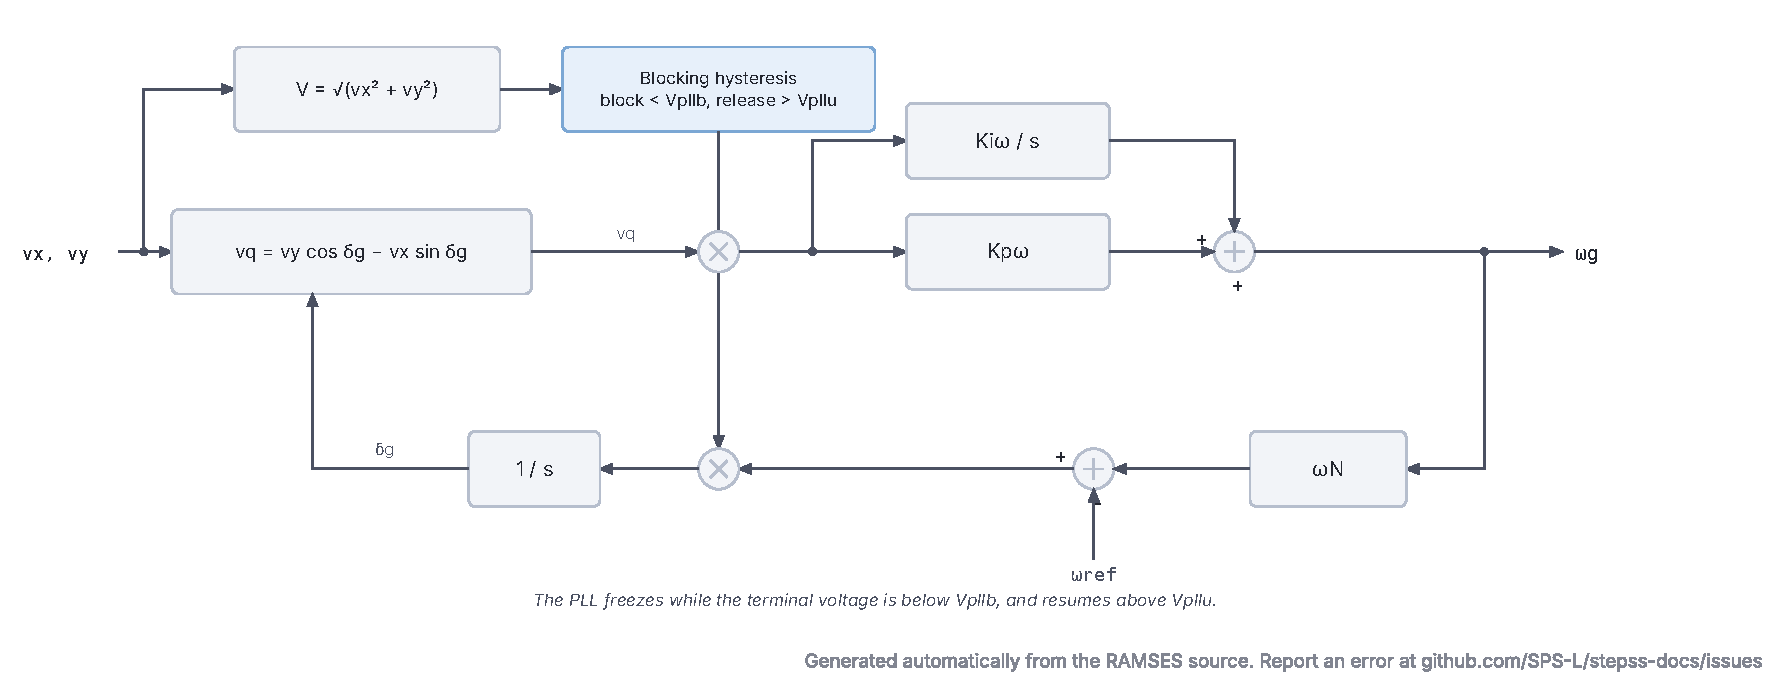
\includegraphics[width=0.98\linewidth]{figures/inj-gfol-pll-light}
\caption{Grid-following phase-locked loop block diagram.}
\end{figure}

The \(q\)-axis voltage error drives a PI controller whose output is the grid frequency estimate \(\tilde{\omega}_g\) (state \texttt{w\_pll}); integrating \(\omega_N(\tilde{\omega}_g - \omega_{\mathrm{ref}})\) gives the PLL angle. The PI gains follow from the PLL response time \(\tau\):

\[K_{p\omega} = \frac{10}{\omega_N \tau}, \qquad K_{i\omega} = \frac{25}{\omega_N \tau^2}, \qquad \omega_N = 2\pi f_N\]

The PLL is blocked once the PCC voltage \(V\) falls below \texttt{Vpllb} and reactivated once \(V\) recovers above \texttt{Vpllu} (hysteresis).

\textbf{Inner current control.}

\begin{figure}[htbp]
\centering
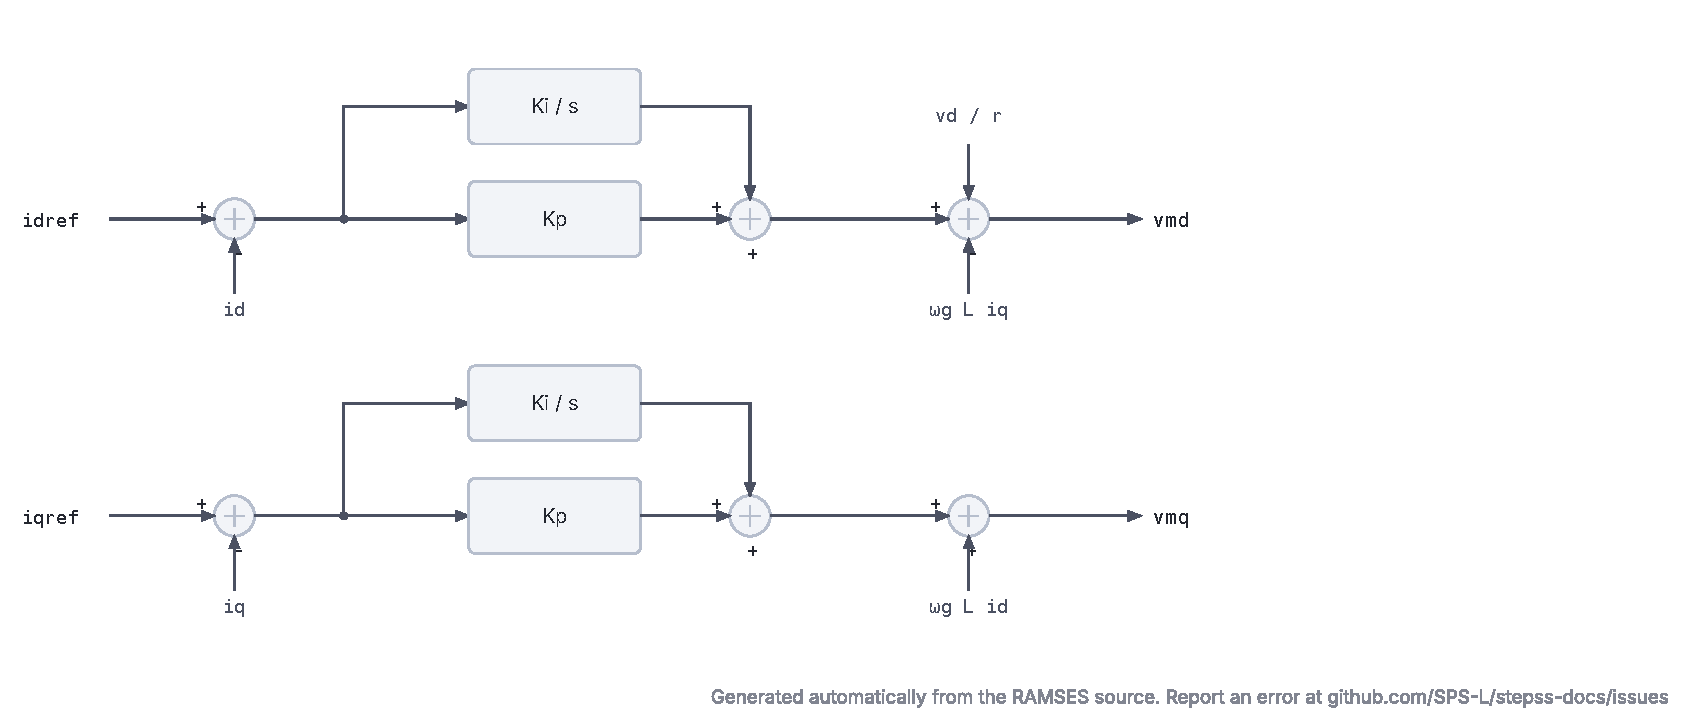
\includegraphics[width=0.98\linewidth]{figures/inj-gfol-currentctl-light}
\caption{Grid-following inner current control.}
\end{figure}

\[v_{md} = \frac{v_d}{r} - \tilde{\omega}_g L\, i_q + \left(K_p + \frac{K_i}{s}\right)\left(i_d^{\mathrm{ref}} - i_d\right)\]

\[v_{mq} = \tilde{\omega}_g L\, i_d + \left(K_p + \frac{K_i}{s}\right)\left(i_q^{\mathrm{ref}} - i_q\right)\]

combined with the transformer voltage-current relationship in the \(d\)-\(q\) frame:

\[v_{md} = \frac{v_d}{r} + R\, i_d - \tilde{\omega}_g L\, i_q, \qquad v_{mq} = \frac{v_q}{r} + R\, i_q + \tilde{\omega}_g L\, i_d\]

\textbf{Active power control.}

\begin{figure}[htbp]
\centering
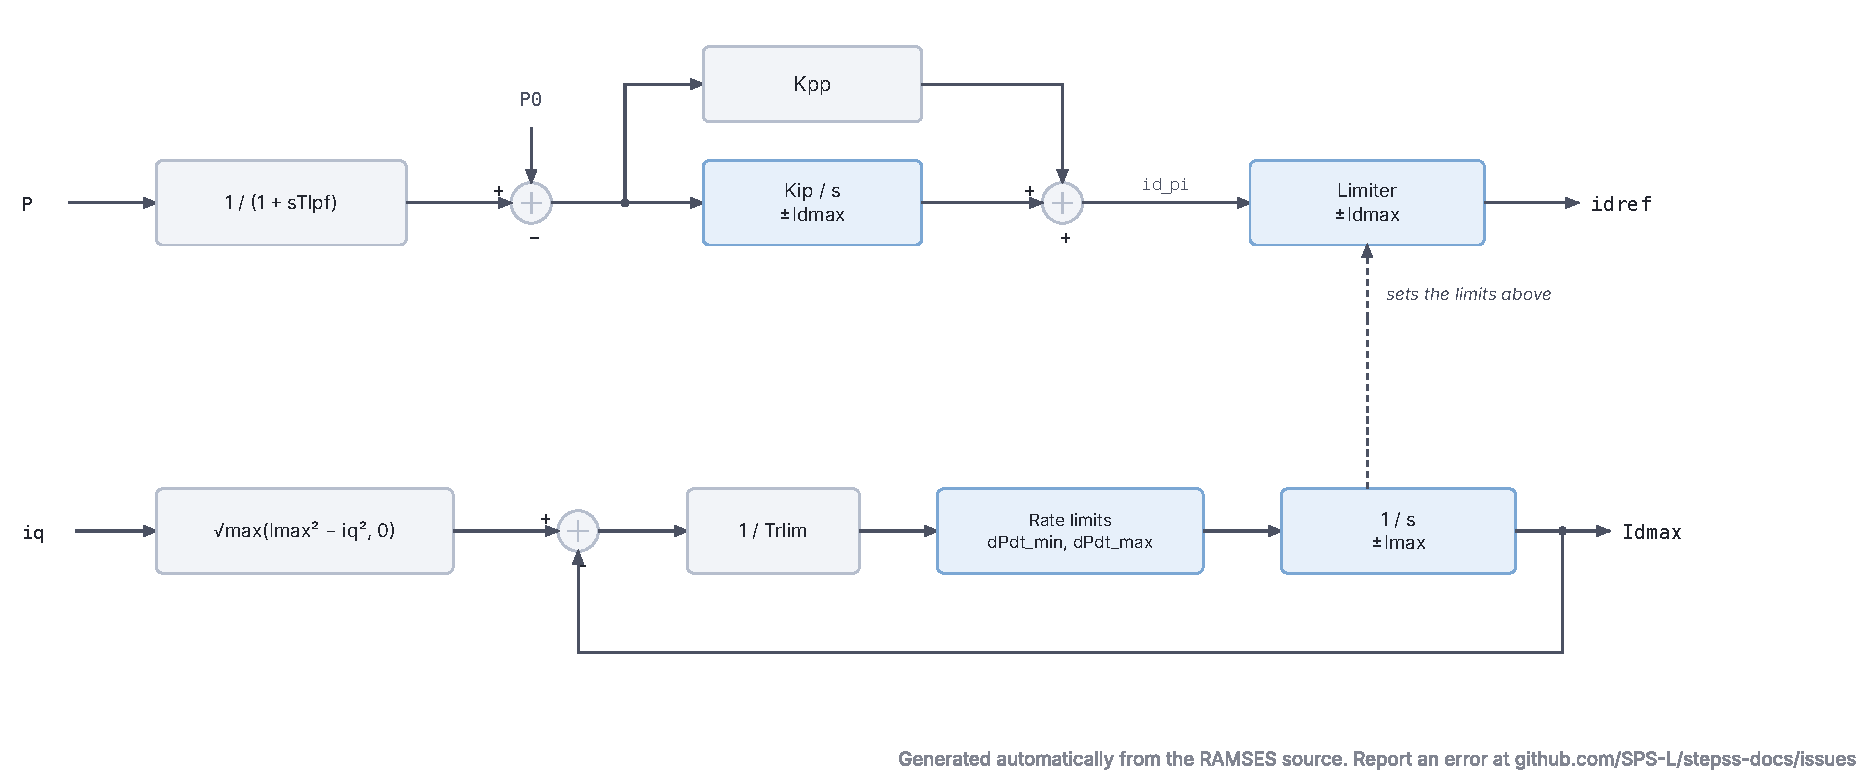
\includegraphics[width=0.98\linewidth]{figures/inj-gfol-pctl-light}
\caption{Grid-following active power control.}
\end{figure}

The measured active power is filtered with time constant \(T_{\mathrm{lpf}}\) and compared with the setpoint \(P^0\); a PI controller (\(K_{pp}\), \(K_{ip}\)) with non-windup limits \(\pm I_d^{\max}\) produces \(i_d^{\mathrm{ref}}\). The limit gives \textbf{priority to the reactive current}:

\[I_d^{\max,\mathrm{stat}} = \sqrt{\max\left(I_{\mathrm{max}}^2 - i_q^2,\; 0\right)}\]

and \(I_d^{\max}\) tracks this static value through a first-order lag (\(T_{\mathrm{rlim}}\), typically 0.002 s) with rate limits \texttt{dPdt\_min}/\texttt{dPdt\_max}, limiting in particular the rate of recovery of the active current after it has been decreased by an increase of \(i_q\).

\textbf{Voltage / reactive power control.}

\begin{figure}[htbp]
\centering
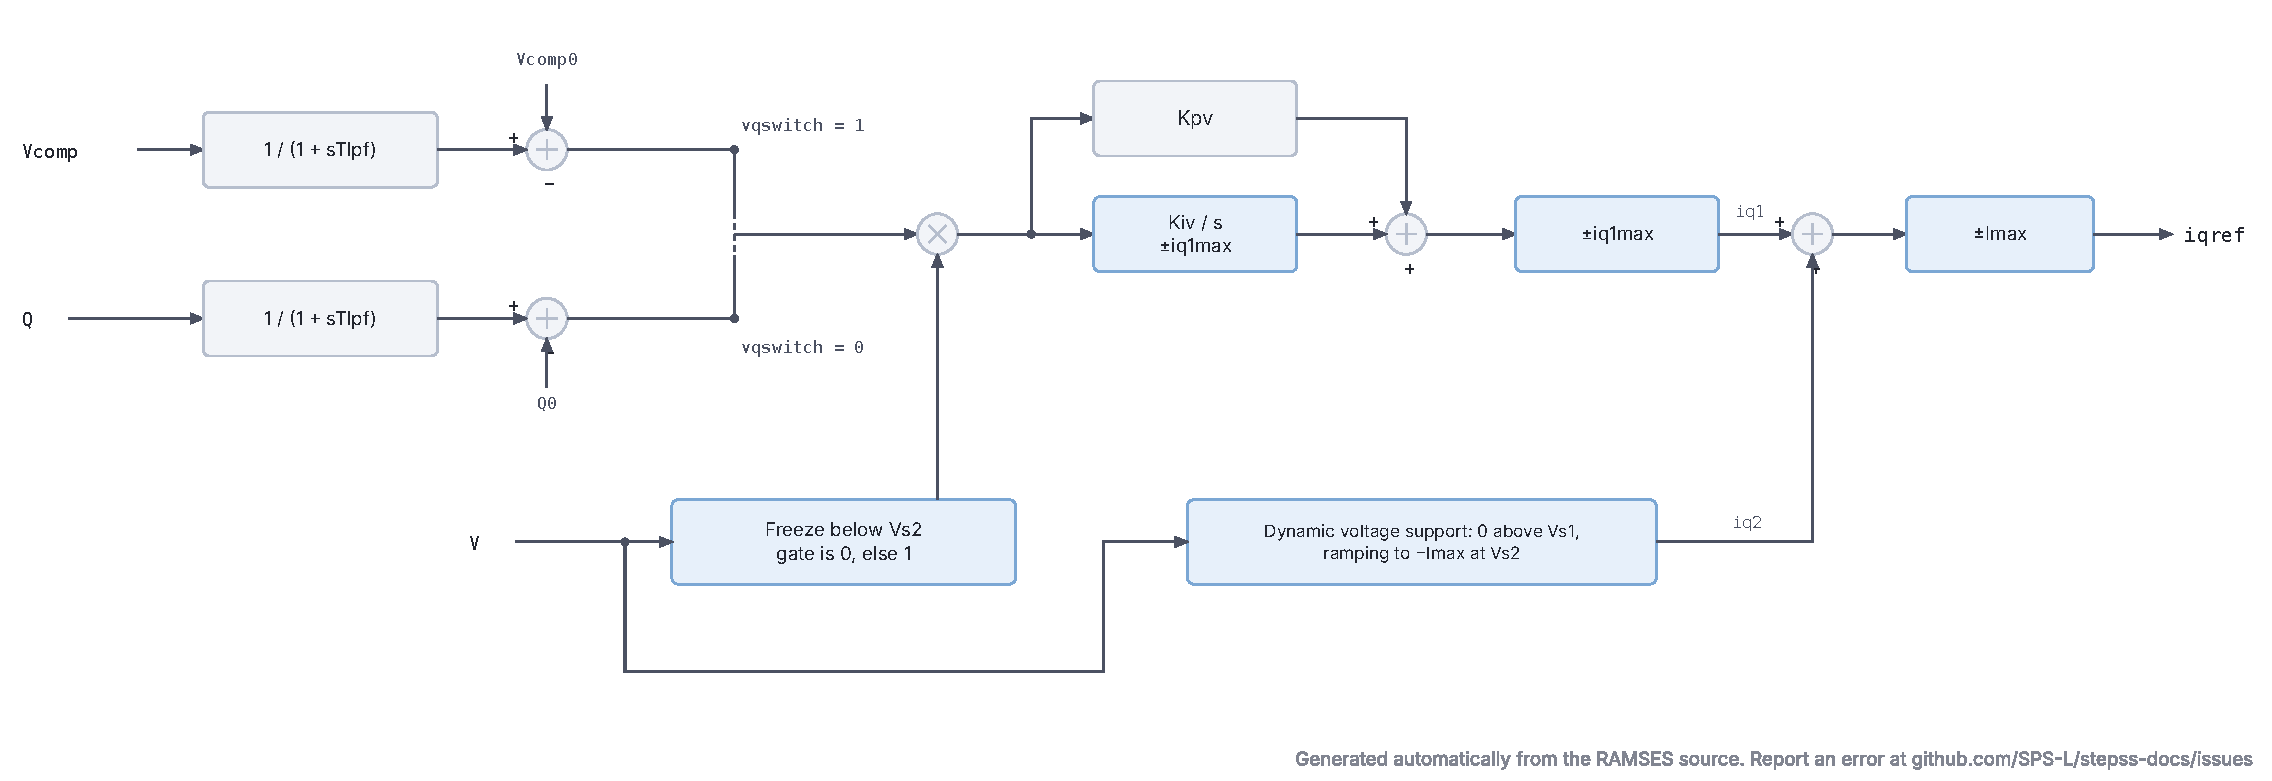
\includegraphics[width=0.98\linewidth]{figures/inj-gfol-qctl-light}
\caption{Grid-following voltage and reactive power control.}
\end{figure}

Depending on \texttt{vqswitch}, either the compensated voltage or the reactive power is controlled:

\[V_c = \left|\frac{\bar{v}}{r} + (R_c + jX_c)\,\bar{i}\right| \quad (\texttt{vqswitch}=1), \qquad Q = \frac{v_q}{r} i_d - \frac{v_d}{r} i_q \quad (\texttt{vqswitch}=0)\]

The controlled quantity is filtered (\(T_{\mathrm{lpf}}\)) and its deviation from setpoint drives a PI controller (\(K_{pv}\), \(K_{iv}\)) with non-windup limits \(\pm i_{q1}^{\max}\), giving the component \(i_{q1}\). The error is zeroed (controller frozen) while \(V < V_{s2}\). A second component \(i_{q2}\) implements dynamic voltage support as a piecewise-linear function of \(V\): zero above \(V_{s1}\), decreasing linearly to \(-I_{\mathrm{max}}\) at \(V_{s2}\), constant below. The total \(i_{q1} + i_{q2}\), limited to \(\pm I_{\mathrm{max}}\), is the reactive current reference \(i_q^{\mathrm{ref}}\).

With \(R_c = R\), \(X_c = \omega L\) and \(r = 1\), controlling \(V_c\) amounts to controlling the magnitude of the modulated voltage.

\subsection{Parameters}\label{model-inj-conv:parameters-2}

Default values correspond to a 1200 MVA converter. Per-unit values refer to the nominal apparent power of the converter.

\begin{small}\begin{longtable}[]{@{}
  >{\raggedright\arraybackslash}p{(\linewidth - 10\tabcolsep) * \real{0.1005}}
  >{\raggedright\arraybackslash}p{(\linewidth - 10\tabcolsep) * \real{0.1524}}
  >{\raggedright\arraybackslash}p{(\linewidth - 10\tabcolsep) * \real{0.4781}}
  >{\raggedright\arraybackslash}p{(\linewidth - 10\tabcolsep) * \real{0.1030}}
  >{\raggedright\arraybackslash}p{(\linewidth - 10\tabcolsep) * \real{0.1659}}
@{}}
\toprule\noalign{}
\begin{minipage}[b]{\linewidth}\raggedright
\#
\end{minipage} & \begin{minipage}[b]{\linewidth}\raggedright
Name
\end{minipage} & \begin{minipage}[b]{\linewidth}\raggedright
Description
\end{minipage} & \begin{minipage}[b]{\linewidth}\raggedright
Unit
\end{minipage} & \begin{minipage}[b]{\linewidth}\raggedright
Default
\end{minipage} \\
\midrule\noalign{}
\endhead
\bottomrule\noalign{}
\endlastfoot
1 & \texttt{R} & Phase reactor resistance & pu & 0.005 \\
2 & \texttt{L} & Phase reactor inductance & pu & 0.15 \\
3 & \texttt{r} & Ratio of ideal transformer & & 1.02 \\
4 & \texttt{Snom} & Nominal apparent power & MVA & 1200 \\
5 & \texttt{Rc} & Resistance used in compensated voltage & pu & 0.005 \\
6 & \texttt{Xc} & Reactance used in compensated voltage & pu & 0.15 \\
7 & \texttt{Kp} & Current control: proportional gain & & 0.573 \\
8 & \texttt{Ki} & Current control: integral gain & & 6.0 \\
9 & \texttt{Tlpf} & Measurement time constant (low-pass filter) & s & 0.0033 \\
10 & \texttt{Kpp} & Active power control: proportional gain & & 0.0333 \\
11 & \texttt{Kip} & Active power control: integral gain & & 10.0 \\
12 & \texttt{Trlim} & Time constant of the \(I_d^{\max}\) rate limiter & s & 0.002 \\
13 & \texttt{dPdt\_min} & Min rate of change of the \(d\)-current limit & pu/s & -999 \\
14 & \texttt{dPdt\_max} & Max rate of change of the \(d\)-current limit & pu/s & 10.0 \\
15 & \texttt{Kpv} & Reactive power control: proportional gain & & 0.1667 \\
16 & \texttt{Kiv} & Reactive power control: integral gain & & 50.0 \\
17 & \texttt{tau} & Response time of PLL & s & 0.10 \\
18 & \texttt{Vpllb} & Voltage below which the PLL is blocked & pu & 0.4 \\
19 & \texttt{Vpllu} & Voltage above which the PLL is unblocked & pu & 0.5 \\
20 & \texttt{Imax} & Maximum current (typically 1--1.2) & pu & 1.0 \\
21 & \texttt{Vs1} & Voltage below which dynamic reactive support starts & pu & -1000 \\
22 & \texttt{Vs2} & Voltage at which reactive support is maximum (\(V_{s2} < V_{s1}\)) & pu & -2000 \\
23 & \texttt{iqmax} & Limit (\ensuremath{\pm}) on quadrature current component \(i_{q1}\) & pu & 1.001 \\
24 & \texttt{vqswitch} & 1 = voltage control, 0 = reactive power control & flag & 1 \\
\end{longtable}\end{small}

Setting \texttt{Vs1} and \texttt{Vs2} to large negative values (as in the defaults above) disables the dynamic voltage support; a more elaborate control is recommended for that function. Typical values of \texttt{Kiv} are 50 pu/s for voltage control and 10 pu/s for reactive power control.

Six additional parameters are computed at initialization from the power-flow solution: \texttt{k} (current conversion factor), \texttt{P0}, \texttt{Q0} (active/reactive power setpoints, pu on \texttt{Snom} base), \texttt{Vc0} (compensated voltage setpoint), \texttt{Imin} and \texttt{iq1max} (\(= \min(\texttt{iqmax}, I_{\mathrm{max}})\)). \texttt{P0}, \texttt{Q0} and \texttt{Vc0} can be modified during the simulation with \texttt{CHGPRM} disturbances.

\subsection{State Variables}\label{model-inj-conv:state-variables-2}

The model has 52 states (2 output currents + 50 internal). Key internal states:

\begin{small}\begin{longtable}[]{@{}
  >{\raggedright\arraybackslash}p{(\linewidth - 6\tabcolsep) * \real{0.2931}}
  >{\raggedright\arraybackslash}p{(\linewidth - 6\tabcolsep) * \real{0.5676}}
  >{\raggedright\arraybackslash}p{(\linewidth - 6\tabcolsep) * \real{0.1393}}
@{}}
\toprule\noalign{}
\begin{minipage}[b]{\linewidth}\raggedright
Variable
\end{minipage} & \begin{minipage}[b]{\linewidth}\raggedright
Description
\end{minipage} & \begin{minipage}[b]{\linewidth}\raggedright
Unit
\end{minipage} \\
\midrule\noalign{}
\endhead
\bottomrule\noalign{}
\endlastfoot
\texttt{wref} & Angular speed of reference axes & pu \\
\texttt{ixt}, \texttt{iyt} & Converter-side currents (on \texttt{Snom} base) & pu \\
\texttt{mult\_pll} & PLL freezing factor (hysteresis output) & \\
\texttt{w\_pll}, \texttt{theta\_pll} & PLL frequency and angle estimates & pu, rad \\
\texttt{V}, \texttt{vd}, \texttt{vq} & PCC voltage magnitude and \(d\)-\(q\) components & pu \\
\texttt{id}, \texttt{iq} & Converter currents in \(d\)-\(q\) frame & pu \\
\texttt{vmd}, \texttt{vmq} & Modulated voltage components & pu \\
\texttt{Md}, \texttt{Mq} & Current-control PI outputs & pu \\
\texttt{Idmax\_stat}, \texttt{Idmax}, \texttt{Idmin} & Static / rate-limited / minimum \(d\)-current limits & pu \\
\texttt{P}, \texttt{Pfil} & Active power and its filtered value & pu \\
\texttt{id\_pi}, \texttt{idref} & Active-power PI output and \(d\)-current reference & pu \\
\texttt{Vc}, \texttt{Vcfil} & Compensated voltage and its filtered value & pu \\
\texttt{Q}, \texttt{Qfil} & Reactive power and its filtered value & pu \\
\texttt{mult\_V} & Voltage/reactive controller freezing factor & \\
\texttt{iq\_1}, \texttt{iq\_2}, \texttt{iqref} & Reactive current components and reference & pu \\
\end{longtable}\end{small}

\textbf{Observables:} \texttt{P\_MW}, \texttt{Q\_Mvar}, \texttt{Vc}, \texttt{Vm}, \texttt{vmd}, \texttt{vmq}, \texttt{I}, \texttt{w\_pll}, \texttt{theta\_pll\_deg}, \texttt{mult\_pll}, \texttt{Idmax}, \texttt{Md}, \texttt{idref}, \texttt{id}, \texttt{id\_pi}, \texttt{iq\_1}, \texttt{iq\_2}, \texttt{iqref}, \texttt{iq}.

\subsection{Usage Example}\label{model-inj-conv:usage-example-3}

A 1200 MVA grid-following converter (record spanning multiple lines):

\begin{Verbatim}
INJEC  GFOL  HVDC1  A
      # FP FQ P Q: share of the power-flow injection (FP, FQ) or initial power (P in MW, Q in Mvar)
      1.  1.  0.  0.
      # R: Phase reactor resistance (pu)
      0.005
      # L: Phase reactor inductance (pu)
      0.15
      # r: Ratio of the ideal connection transformer (pu/pu)
      1.02
      # Snom: Nominal apparent power (MVA)
      1200.
      # Rc: Resistance used in compensated voltage (pu)
      0.005
      # Xc: Reactance used in compensated voltage (pu)
      0.15
      # Kp: Current control: proportional gain
      0.5730
      # Ki: Current control: integral gain
      6.
      # Tlpf: Measurement time constant (low-pass filter) (s)
      0.0033
      # Kpp: Active power control: proportional gain
      0.0333
      # Kip: Active power control: integral gain
      10.
      # Trlim: Time constant of the I_d^max rate limiter (s)
      0.002
      # dPdt_min: Min rate of change of the d-current limit (pu/s)
      -999.
      # dPdt_max: Max rate of change of the d-current limit (pu/s)
      10.
      # Kpv: Reactive power control: proportional gain
      0.1667
      # Kiv: Reactive power control: integral gain
      50.
      # tau: Response time of PLL (s)
      0.10
      # Vpllb: Voltage below which the PLL is blocked (pu)
      0.4
      # Vpllu: Voltage above which the PLL is unblocked (pu)
      0.5
      # Imax: Maximum current (typically 1-1.2) (pu)
      1.000
      # Vs1: Voltage below which dynamic reactive support starts (pu)
      -1000
      # Vs2: Voltage below which reactive support is maximum and the V/Q PI is frozen (pu)
      -2000
      # iqmax: Limit (+/-) on quadrature current component i_q1 (pu)
      1.001
      # vqswitch: 1 = voltage control, 0 = reactive power control (flag)
      1
;
\end{Verbatim}
